\documentclass[11pt,a4paper]{article}

% ---------- Packages ----------
\usepackage[utf8]{inputenc}
\usepackage[T1]{fontenc}
\usepackage{lmodern}
\usepackage[english]{babel}
\usepackage[a4paper,margin=2.5cm]{geometry}
\usepackage{amsmath, amssymb, amsthm}
\usepackage{graphicx}
\usepackage{booktabs}
\usepackage{caption}
\usepackage{subcaption}
\usepackage{float}
\usepackage{microtype}
\usepackage[round, authoryear]{natbib}
\usepackage{hyperref}
\usepackage{url}
\usepackage{xcolor}
\usepackage{enumitem}
\usepackage{fontawesome5}

% Repository link, surfaced near the title for one-click access.
\newcommand{\repolink}{\href{https://github.com/lukaschudy/thesis}{\faGithub\ \textsf{Code on GitHub}}}

% Draft-mode marginal note macro for tentative claims, references to verify,
% etc. They render as inline footnotes in the draft and can be turned off
% by switching the definition to \newcommand{\todo}[1]{}.
\newcommand{\todo}[1]{\footnote{\textcolor{red}{\textbf{[draft note]} #1}}}

\hypersetup{
    colorlinks=true,
    linkcolor=black,
    citecolor=blue!60!black,
    urlcolor=blue!60!black
}

% ---------- Math shortcuts ----------
\newcommand{\R}{\mathbb{R}}
\newcommand{\E}{\mathbb{E}}
\newcommand{\Pnash}{\pi^{\mathrm{N}}}
\newcommand{\Pmono}{\pi^{\mathrm{M}}}

% ---------- Title ----------
\title{
    \vspace{-1.5cm}
    \textbf{Robustness of Algorithmic Collusion to Information and Timing Frictions in Q-Learning Pricing} \\
    \vspace{0.3cm}
    \large{\textit{Working draft}} \\
    \vspace{0.3cm}
    \normalsize{\repolink}
}
\author{Luk\'a\v{s} Chud\'y}
\date{\today}

\begin{document}
\maketitle

\begin{abstract}
\noindent
Independent tabular Q-learning pricing agents in a repeated Bertrand duopoly are known to converge on supracompetitive prices without explicit communication \citep{calvano2020}. The literature has so far studied this phenomenon under idealised informational and timing assumptions: instantaneous and noiseless observation of the rival's price, and simultaneous price-setting each period. This paper relaxes those assumptions one at a time and then in combination. Three frictions are introduced into the otherwise unchanged \citet{calvano2020} environment: (i) \emph{observation latency}, where each agent observes the rival's price with a delay of $L$ periods; (ii) \emph{noisy monitoring}, where the rival's observed price is corrupted by Gaussian measurement error of standard deviation $\sigma$; and (iii) \emph{asynchronous actions} in the Maskin--Tirole sense, where only one agent revises its price per $T$-period block. The single-friction sweeps reveal three qualitatively different shapes of the collusion-vs-friction relationship: latency exhibits a sharp cliff at $L=1$ followed by a residual collusion floor of about $\Delta\approx 0.16$; noise produces a smooth monotone decline that reaches Nash by $\sigma=5$; asynchrony reduces $\Delta$ from $0.84$ to $\approx 0.40$ at $T=1$ and then plateaus. A $2\times 2\times 2$ factorial experiment, replicated at $250$, $500$ and $1000$ sessions, examines whether the frictions interact. Two robust interaction patterns emerge: latency and noise compound super-multiplicatively, and asynchrony partially \emph{rescues} collusion when imposed on top of either of the other two frictions. The latter result is the opposite-sign of the main effect of asynchrony alone, and suggests that mandatory staggered-pricing rules and information-degradation rules are policy substitutes rather than complements.

\end{abstract}

\section{Introduction}
\label{sec:introduction}

The practical policy concern behind this thesis is not simply that pricing algorithms can raise prices in a laboratory model. It is whether the messy information and timing conditions of real markets make that concern smaller or larger. Algorithmic pricing is already discussed by competition authorities in sectors such as travel, entertainment, retail, and fuel, and empirical work studies its effects in online retail and German petrol markets \citep{oecd2025,brown2023,assad2024}. In the German petrol market, for example, \citet{assad2024} find that markups rose around the time major chains adopted algorithmic pricing software. These markets do not look like frictionless textbook games. Firms observe rivals through booking systems, web scrapers, price feeds, shelf tags, and reporting platforms, all of which can be delayed, noisy, or tied to fixed update schedules. If those frictions already weaken algorithmic collusion, then the policy problem is less urgent than the clean simulation literature suggests. If they can instead preserve or even restore collusion when combined, then the problem is larger than one would infer from studying each friction in isolation.

The legal difficulty is that cartel enforcement is built around agreement. Explicit price fixing is illegal because it raises prices above the competitive level, transfers surplus from consumers to firms, and creates deadweight loss \citep{businessgovnl}. But autonomous algorithmic coordination may not involve the kind of communication, meeting of minds, or explicit agreement that competition law is normally designed to prove. The OECD therefore treats algorithmic collusion as a challenge for traditional concepts of agreement and tacit coordination \citep{oecd2017,oecd2025}. \citet{calvano2020} make the concern concrete: two independent Q-learning algorithms in a repeated pricing game learn prices about 84\% of the way from competitive Nash to joint monopoly, without ever communicating. In economic terms the outcome resembles a cartel, but the conduct is generated by trial-and-error learning rather than an explicit agreement. The full literature, including the follow-up simulation studies and the empirical evidence, is reviewed in Section~\ref{sec:literature}.

The natural next question is whether the Calvano result survives once the information environment becomes less clean. This matters both descriptively and for policy. Descriptively, real pricing algorithms do not always see rival prices instantly or perfectly. They often receive stale, rounded, scraped, or otherwise imperfect signals. For policy, these same features are possible indirect levers: a regulator may not be able to prosecute communication-free learning directly, but could still ask whether delayed disclosure, noisy public price feeds, or commitment windows would make algorithmic coordination less likely. Existing papers study some of these channels one at a time. What is less clear is whether they still work when imposed together, or whether one friction can undo the effect of another.

I keep the \citet{calvano2020} pricing environment fixed and change only the way the algorithms observe or time their decisions. In the baseline, two firms repeatedly choose prices, consumers respond according to logit demand, and each firm is controlled by a Q-learning algorithm that learns from its own profits and the rival's previous price. I measure the outcome using the profit-gain index $\Delta$. This is an economic collusion score: $\Delta=0$ means profits are at the competitive Nash benchmark, while $\Delta=1$ means profits are at the joint-monopoly benchmark. A value such as $\Delta=0.5$ therefore means that the algorithms have recovered about half of the profit gap between competition and joint monopoly, which is already a substantial supracompetitive outcome. The thesis asks how this score changes when three frictions are introduced separately and jointly:
\begin{enumerate}[label=\textbf{RQ\arabic*.}, leftmargin=3em, labelsep=0.6em, itemsep=5pt, parsep=0pt, topsep=10pt, partopsep=3pt]
    \item How does observation latency (delayed observation of the rival's price) affect collusion?
    \item How does noisy monitoring (Gaussian misobservation of the rival's price) affect collusion?
    \item How does asynchronous price setting (Maskin--Tirole alternation between movers) affect collusion?
    \item Do these frictions interact non-linearly when imposed jointly?
\end{enumerate}

Varying each friction separately gives three different response patterns in the collusion score: latency produces a sharp initial drop, noise produces a smooth decline toward the competitive benchmark, and asynchrony produces a one-time drop followed by a plateau. A $2\times 2\times 2$ factorial experiment, replicated at three session counts to confirm robustness, then identifies two interaction patterns. Latency and noise compound: imposing both jointly destroys more collusion than independent dampening would predict, because the two frictions degrade different dimensions of the rival's observation, timing and value. Asynchrony has the opposite interaction. Although it reduces collusion on its own, it partially restores collusion when combined with latency or noise. The policy relevance is therefore cautious rather than prescriptive. The results do not say that a particular regulatory package should be adopted. They show that the case for intervention cannot be assessed by testing one friction at a time, because realistic combinations can amplify some anti-collusion effects while offsetting others.

\section{Methodology}
\label{sec:methodology}

This section sets out the baseline environment, the three friction extensions, and the unified factorial implementation. It also flags, in each subsection, every place where the implemented design departs from what the proposal specified, with a brief justification.\todo{Make sure the methodology is read in the order: baseline $\to$ each friction $\to$ unified design. The deviations from the proposal --- noise distribution, async schedule, off-path tests --- are flagged inline; consider whether to also collect them in a single ``deviations from the proposal'' table at the end of this section.}

\subsection{Baseline environment}
\label{sec:methodology-baseline}

The baseline reproduces \citet{calvano2020}. Two firms (\(n=2\)) repeatedly play a Bertrand pricing game with logit demand. The action set is a discrete grid of \(m=15\) prices, constructed by taking the static-Bertrand Nash and the (symmetric) joint-monopoly prices and extending the range slightly above and below them. Demand has the standard logit form
\begin{equation}
    q_i(p_1, p_2) \;=\; \frac{\exp\!\left(\frac{a_i - p_i}{\mu}\right)}{\sum_{j=1}^{n}\exp\!\left(\frac{a_j - p_j}{\mu}\right) + \exp\!\left(\frac{a_0}{\mu}\right)},
    \label{eq:logit-demand}
\end{equation}
with vertical-quality parameters \(a_1 = a_2 = 2\), outside-option \(a_0=0\), and horizontal-differentiation parameter \(\mu = 0.25\). Marginal costs are \(c_1 = c_2 = 1\). Single-period profits are \(\pi_i(p_1,p_2) = (p_i - c_i)\,q_i(p_1,p_2)\).

The state at time \(t\) is the vector of last-period prices \(s_t = (p_{1,t-1}, p_{2,t-1})\), so memory length \(k=1\). With \(m\) price levels per agent the state space has \(m^{2}\) elements. Each agent maintains a tabular action-value function \(Q_i: \mathcal{S}\times\mathcal{A}_i \to \R\). Actions are selected by an \(\varepsilon\)-greedy rule with exponentially decaying exploration:
\begin{equation}
    a_{i,t} \;=\; \begin{cases} \mathrm{argmax}_{a}\, Q_{i,t}(s_t,a) & \text{with probability } 1-\varepsilon_t,\\ \mathrm{Uniform}(\mathcal{A}_i) & \text{with probability } \varepsilon_t,\end{cases} \qquad \varepsilon_t = e^{-\beta\,t}.
\end{equation}
The Q-table updates are the standard one-step Q-learning rule
\begin{equation}
    Q_{i,t+1}(s_t, a_{i,t}) \;=\; (1-\alpha)\,Q_{i,t}(s_t,a_{i,t}) \;+\; \alpha\!\left[\pi_i(a_t) + \delta\,\max_{a'}Q_{i,t}(s_{t+1}, a')\right],
    \label{eq:Q-update}
\end{equation}
with learning rate \(\alpha = 0.15\) and discount factor \(\delta = 0.95\). The exploration parameter is \(\beta = 4\times 10^{-6}\), implemented as a per-episode multiplier \(\varepsilon_{\text{decay}}=0.02\) over episodes of length \(5{,}000\) iterations.

A run is a sequence of one or more \emph{sessions}. Each session draws fresh random initial Q-values and initial prices, and is run until the greedy strategy is unchanged for four consecutive episodes (the standard convergence criterion in this literature) or a 1{,}000-episode cap is reached. Reported quantities are means across sessions of session-level converged values. The primary outcome variable is the average profit gain
\begin{equation}
    \Delta \;=\; \frac{\bar{\pi} - \Pnash}{\Pmono - \Pnash},
\end{equation}
which equals \(0\) when the agents play the static-Bertrand Nash equilibrium and \(1\) when they play the symmetric joint-monopoly prices. We also report the cross-session standard deviation of session-level \(\Delta\) (denoted SD throughout) as a measure of dispersion.

\paragraph{Implementation and validation.}
The simulator is a from-scratch C++17 translation of the Calvano Fortran reference code. The translation was validated against the Fortran output at \(m=15\) before any frictions were introduced, and produces \(\Delta = 0.848\) (1{,}000 sessions, all converged), within sampling noise of \citet{calvano2020}'s reported value of approximately \(0.84\). A grid-robustness check at \(m\in\{15, 25, 50, 100\}\) confirms the result is not a coarse-grid artefact: \(\Delta\) declines mildly from $0.848$ at \(m=15\) to \(0.706\) at \(m=100\) and is essentially flat between \(m=50\) and \(m=100\). All runs use Calvano's original fixed-\(\beta\) protocol; the \(\nu\)-corrected version that holds learning quality constant across \(m\) is left for future work.

\subsection{Friction 1: observation latency}
\label{sec:methodology-latency}

Agent \(i\) at time \(t\) observes the rival's price from period \(t-1-L\) instead of \(t-1\). The own-price observation is unchanged. The agent's perceived state is therefore \(\tilde{s}^{(i)}_t = (p_{i,t-1},\, p_{j,t-1-L})\), which differs across agents whenever \(L\geq 1\). All other elements of the algorithm --- action selection, reward, Q-update, convergence test --- are applied to the per-agent perceived state. Profits are computed from the \emph{true} joint action, so the friction degrades information without altering payoffs.

A per-agent FIFO buffer of length \(L+1\) tracks each agent's price history, initialised by repeating each agent's randomly drawn initial price across the buffer slots. Because exploration is near-uniform during the first \(L\) iterations of every session (\(\varepsilon\approx 1\)) the buffer initialisation has negligible effect. At \(L=0\) the buffer reduces to a single slot and the entire learner reproduces the baseline bit-for-bit, providing an internal sanity check that confirms correctness of the implementation before each parameter sweep.

\subsection{Friction 2: noisy monitoring}
\label{sec:methodology-noise}

Each period, each agent observes the rival's previous-period price corrupted by an independent Gaussian draw on the \emph{price index}:
\begin{equation}
    \tilde{p}^{(i)}_{j,t-1} \;=\; \mathrm{clamp}\!\left(\,\mathrm{round}\!\left(k_{j,t-1} + \sigma\,\varepsilon^{(i)}_t\right),\; 1,\; m\right),
    \qquad \varepsilon^{(i)}_t \sim \mathcal{N}(0,1),
    \label{eq:noise}
\end{equation}
where \(k_{j,t-1}\in\{1,\dots,m\}\) is the rival's true price index and \(\sigma\) is the noise scale. The agent uses the noisy observation as the rival-side coordinate of its perceived state and cannot ``denoise''; noise is drawn independently per agent and per period. Profits are computed from the true joint action.

The proposal originally specified a discrete-flip noise model (probability \(q\) of perturbation to a neighbouring grid point); the implemented Gaussian-on-index version is a smooth one-parameter generalisation, locality-preserving, and reduces to the no-noise baseline at \(\sigma=0\). At \(\sigma=0\) the noise random number generator is short-circuited so the baseline is reproduced bit-for-bit, an internal sanity check parallel to the latency one.

\subsection{Friction 3: asynchronous actions}
\label{sec:methodology-async}

This friction implements the Maskin--Tirole alternating-move structure with a tunable lock-in length \(T\). At every iteration \(t\geq 1\) exactly one agent ``moves'' (revises its price) and the other holds its previous-period price. The mover identity follows a strict deterministic schedule:
\begin{equation}
    \mathrm{mover}(t) \;=\; \left(\!\left\lfloor \tfrac{t-1}{T} \right\rfloor \!\bmod\! 2\right) + 1.
\end{equation}
At \(T=0\) the rule is short-circuited and both agents move every period, recovering the simultaneous baseline. At \(T=1\) the agents strictly alternate (the standard Maskin--Tirole case). At \(T=k\) the moving agent is locked in for \(k\) consecutive periods before the other agent takes over.

Both agents Q-learn every period regardless of who moved. The non-mover's ``action'' is its previous-period price (a valid element of its action set), and its Q-update uses the observed reward from the actual joint action just like the mover's. The exploration parameter \(\varepsilon_t\) decays for both agents every period, on the convention that one iteration is one unit of calendar time for everyone.

The proposal originally suggested random alternation plus off-path deviation tests; the implemented version uses strict deterministic alternation and varies \(T\) on a grid. Off-path deviation analysis is left for future work.

\subsection{Combined frictions}
\label{sec:methodology-combined}

To test whether the three frictions interact, a \emph{unified} learner accepts \((L, \sigma, T)\) jointly and applies all three simultaneously. Within each iteration the order of operations is:
\begin{enumerate}[itemsep=0pt, topsep=2pt]
    \item Each agent's perceived state is \(\tilde{s}^{(i)}_t = (p_{i,t-1},\, \mathrm{noise}(p_{j,t-1-L}))\) --- noise is applied to the already-lagged observation.
    \item The mover (under \(T\)-period lock-in) is determined; the non-mover's action equals its previous-period price.
    \item The mover selects an action via \(\varepsilon\)-greedy on its own perceived state.
    \item Profits are computed from the true joint action.
    \item Both agents Q-update on their own perceived current and next-period state.
    \item Price-history buffers and \(\varepsilon\) decay one step.
\end{enumerate}
At \((L=0,\sigma=0,T=0)\) the unified learner reproduces the baseline. At single-friction corners it reproduces the corresponding single-friction learner to numerical precision. These two correspondences serve as built-in cross-validation tests of the unified implementation against each of the three single-friction implementations.

\paragraph{Factorial design.}
The factorial uses two levels per friction: ``off'' (the friction's null value) and ``on'' (a moderate, non-saturating value). The on-levels are chosen so that each single-friction effect is visible but not at the floor:
\begin{itemize}[itemsep=0pt, topsep=2pt]
    \item \(L \in \{0, 2\}\) --- at \(L=2\) the latency-only \(\Delta\) is approximately \(0.215\) (a \(75\%\) reduction).
    \item \(\sigma \in \{0, 1\}\) --- at \(\sigma=1\) the noise-only \(\Delta\) is approximately \(0.493\) (a \(42\%\) reduction).
    \item \(T \in \{0, 1\}\) --- at \(T=1\) the async-only \(\Delta\) is approximately \(0.378\) (a \(55\%\) reduction).
\end{itemize}
The eight cells are labelled \texttt{F$abc$} where each digit \(a,b,c\in\{0,1\}\) indicates whether \(L\), \(\sigma\), \(T\) is on. Each cell is run at \(N=250, 500, 1000\) sessions to verify that the interaction pattern is not an artefact of replication noise.

\paragraph{Session counts and standard errors.}
The single-friction sweeps and the \(N=250\) factorial use 250 sessions per cell. The factorial replications add 500 and 1000 sessions per cell. The reported SD is the standard deviation of session-level \(\Delta\) values across sessions; the standard error of the mean scales as \(\mathrm{SD}/\sqrt{N}\), and is below \(0.02\) on the headline factorial cells at \(N=1000\), tight enough to distinguish the three benchmark predictions in Section~\ref{sec:results-factorial}.

\section{Results: single-friction sweeps}
\label{sec:results-singles}

This section reports the three single-friction parameter sweeps. Each cell uses 250 sessions of the unified C++ simulator described in Section~\ref{sec:methodology}; reported numbers are means of converged session-level $\Delta$ with cross-session standard deviation in parentheses. All runs converged --- not a single session failed the four-consecutive-episode strategy-stability test within the 1{,}000-episode cap.

\subsection{Friction 1: observation latency}
\label{sec:results-latency}

Table~\ref{tab:latency-results} reports $\Delta$ across the latency grid \(L\in\{0,1,2,3,5,10,20\}\). At \(L=0\) the simulator reproduces the baseline ($\Delta = 0.843$, SD $= 0.114$), confirming the per-agent state implementation reduces correctly to the shared-state baseline. From \(L=0\) to \(L=1\), $\Delta$ collapses from $0.843$ to $0.280$, a sixty-seven-percent reduction from a single period of observation delay. From \(L=1\) onward, $\Delta$ decays further but more slowly, settling near a floor of approximately $0.16$ for \(L\geq 5\). Figure~\ref{fig:latency} plots the curve.

\begin{table}[H]
\centering
\caption{Effect of observation latency on collusion (250 sessions per cell).}
\label{tab:latency-results}
\begin{tabular}{rcc}
\toprule
$L$ (periods) & $\Delta$ & SD \\
\midrule
0  & 0.843 & 0.114 \\
1  & 0.280 & 0.146 \\
2  & 0.215 & 0.110 \\
3  & 0.193 & 0.088 \\
5  & 0.174 & 0.072 \\
10 & 0.158 & 0.054 \\
20 & 0.155 & 0.052 \\
\bottomrule
\end{tabular}
\end{table}

\begin{figure}[H]
\centering
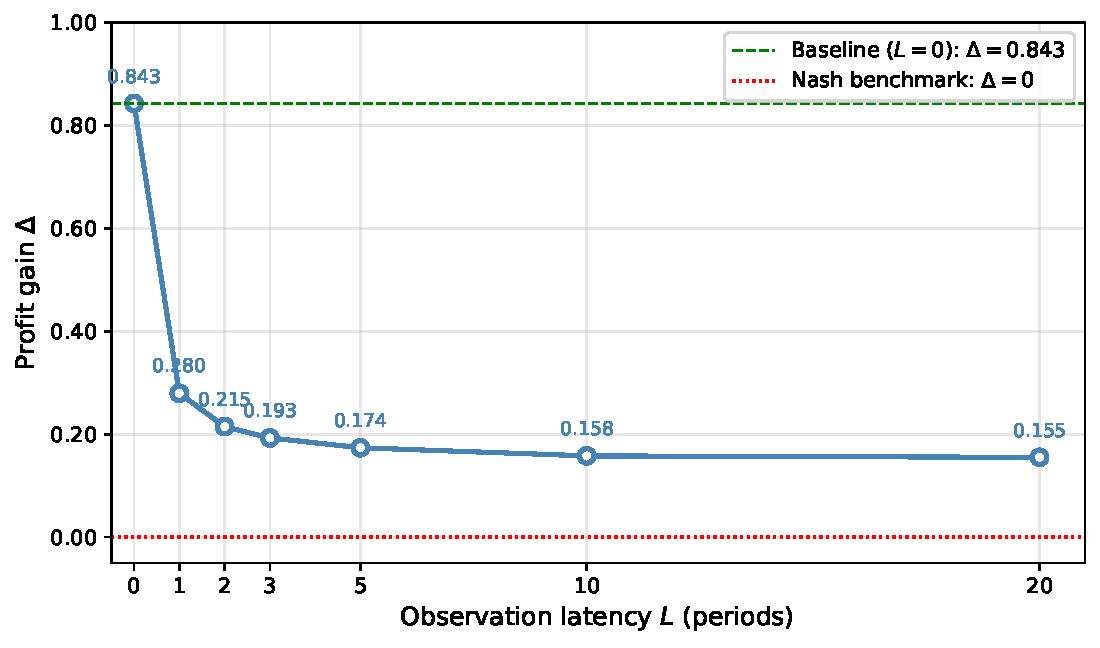
\includegraphics[width=0.78\linewidth]{figures/fig_latency.pdf}
\caption{$\Delta$ as a function of observation latency $L$. The cliff at $L=1$ accounts for nearly the entire effect; further latency adds little.}
\label{fig:latency}
\end{figure}

\paragraph{Interpretation.}
Two features of this curve are worth highlighting. First, the size of the drop at $L=1$ is striking: a single period of delay erases two-thirds of the collusion. The mechanism is that the Calvano baseline relies on the rival's last-period price both as a coordination device and as the input to any retaliation rule. A one-period delay simultaneously breaks both functions. Second, $\Delta$ does not reach Nash even at $L=20$, when an agent is essentially blind for twenty periods. The residual collusion at $\Delta\approx 0.16$ must rest on coordination mechanisms that do \emph{not} require timely monitoring --- most plausibly, agents converge on a stable mutual-high-price focal point that requires no real-time enforcement. This residual is destroyed in Section~\ref{sec:results-noise} when the friction acts on the state \emph{value} rather than on its arrival time.

\subsection{Friction 2: noisy monitoring}
\label{sec:results-noise}

Table~\ref{tab:noise-results} reports $\Delta$ across the noise grid \(\sigma\in\{0, 0.5, 1, 2, 3, 5, 10\}\). At \(\sigma=0\) the result matches the baseline to five decimal places, the bit-for-bit sanity check described in Section~\ref{sec:methodology-noise}. From there $\Delta$ declines smoothly and roughly monotonically: $0.670$ at $\sigma=0.5$, $0.493$ at $\sigma=1$, $0.242$ at $\sigma=2$, falling to essentially Nash ($\Delta=0.013$) by $\sigma=5$. At $\sigma=10$ --- where the noise standard deviation exceeds the entire 15-point price grid and observation is effectively uniform random --- $\Delta=-0.003$, indistinguishable from the Nash benchmark.

\begin{table}[H]
\centering
\caption{Effect of noisy monitoring on collusion (250 sessions per cell).}
\label{tab:noise-results}
\begin{tabular}{rcc}
\toprule
$\sigma$ & $\Delta$ & SD \\
\midrule
0.0  & $\phantom{-}0.843$ & 0.114 \\
0.5  & $\phantom{-}0.670$ & 0.226 \\
1.0  & $\phantom{-}0.493$ & 0.290 \\
2.0  & $\phantom{-}0.242$ & 0.262 \\
3.0  & $\phantom{-}0.143$ & 0.218 \\
5.0  & $\phantom{-}0.013$ & 0.064 \\
10.0 & $-0.003$           & 0.073 \\
\bottomrule
\end{tabular}
\end{table}

\begin{figure}[H]
\centering
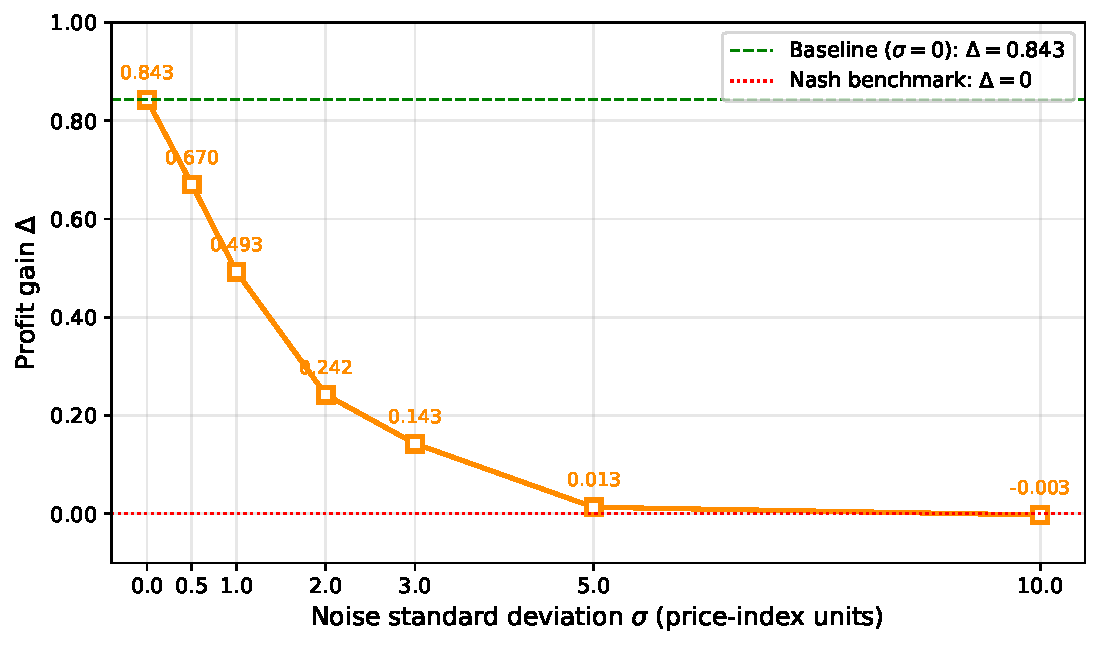
\includegraphics[width=0.78\linewidth]{figures/fig_noise.pdf}
\caption{$\Delta$ as a function of noise standard deviation $\sigma$. Smooth monotone decline; no residual collusion floor.}
\label{fig:noise}
\end{figure}

\paragraph{Interpretation.}
The shape of the noise curve differs from the latency curve in two respects. There is no cliff: the decline from $\Delta=0.843$ to $\Delta\approx 0$ unfolds smoothly across the range $\sigma\in[0,5]$. And there is no residual collusion floor: $\Delta$ at high $\sigma$ converges to the Nash benchmark, not to the $\approx 0.16$ floor seen under heavy latency. The mechanism story is that noise corrupts the \emph{value} of the rival-side state, not its time of arrival. At high $\sigma$ the agent's perceived state is near-independent of the rival's actual price, which means no policy conditioned on that state can encode coordination of any kind, focal or otherwise. Latency leaves the focal-point mechanism intact (the state is correct, just stale); noise destroys it.

The contrast already suggests that the two frictions act through different channels and therefore could compound, the question taken up in Section~\ref{sec:results-factorial}.

\subsection{Friction 3: asynchronous actions}
\label{sec:results-async}

Table~\ref{tab:async-results} reports $\Delta$ across the lock-in grid \(T\in\{0,1,2,5,10,20\}\). At $T=0$ the simulator reproduces the baseline. At $T=1$ --- pure Maskin--Tirole strict alternation --- $\Delta$ drops to $0.378$. From $T=2$ onward the curve plateaus around $\Delta\approx 0.41$, with no further systematic movement up to $T=20$.

\begin{table}[H]
\centering
\caption{Effect of asynchronous actions on collusion (250 sessions per cell).}
\label{tab:async-results}
\begin{tabular}{rcc}
\toprule
$T$ (lock-in length) & $\Delta$ & SD \\
\midrule
0  & 0.843 & 0.114 \\
1  & 0.378 & 0.108 \\
2  & 0.418 & 0.095 \\
5  & 0.424 & 0.116 \\
10 & 0.411 & 0.108 \\
20 & 0.403 & 0.119 \\
\bottomrule
\end{tabular}
\end{table}

\begin{figure}[H]
\centering
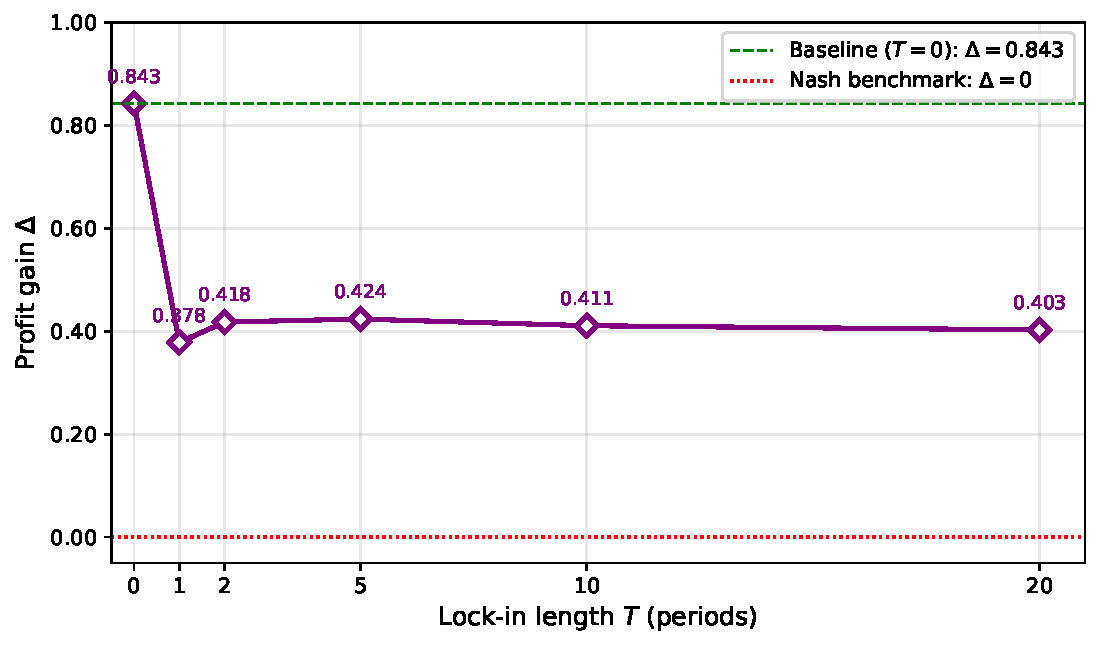
\includegraphics[width=0.78\linewidth]{figures/fig_async.pdf}
\caption{$\Delta$ as a function of asynchrony lock-in length $T$. Step from baseline at $T=0$ to a plateau around $\Delta\approx 0.41$ for $T\geq 1$.}
\label{fig:async}
\end{figure}

\paragraph{Interpretation.}
This curve was the most surprising of the three. The pre-experiment hypothesis, motivated by Maskin--Tirole reaction-function reasoning and \citet{klein2021}'s sequential-pricing results, was that strict alternation should preserve or even enhance collusion: the moving agent faces a known, committed rival price and ought to be able to rationalise a cooperative best-response. The Q-learners do not behave that way at this parameter regime. Mandatory alternation cuts $\Delta$ in roughly half, from $0.843$ to $0.378$ at $T=1$. The plateau at $\Delta\approx 0.41$ for $T\geq 2$ shows that the effect is structural --- it depends on \emph{whether} prices are simultaneous or staggered, not much on \emph{how staggered} they are.

A possible mechanism: under strict alternation, each agent's relevant state-decision pair is restricted to half the periods (only those in which it moves). With $\varepsilon$-greedy exploration and a fixed 5{,}000-iteration episode length, this halves the effective state-visitation rate during learning, and the algorithm has correspondingly more difficulty discovering the high-price equilibria of the baseline. This is a learning-side rather than a strategic-side explanation, distinct from the analytic Maskin--Tirole prediction. Distinguishing the two would require off-path deviation analysis (does the asynchronous equilibrium support punishment? does it survive the genuine-vs-spurious test of \citet{calvano2023}?), which is left to future work.

\subsection{Three shapes side by side}
\label{sec:results-three-comparison}

Figure~\ref{fig:three-friction} places the three single-friction sweeps on a shared $\Delta$ axis. The qualitative differences are visible at a glance.

\begin{figure}[H]
\centering
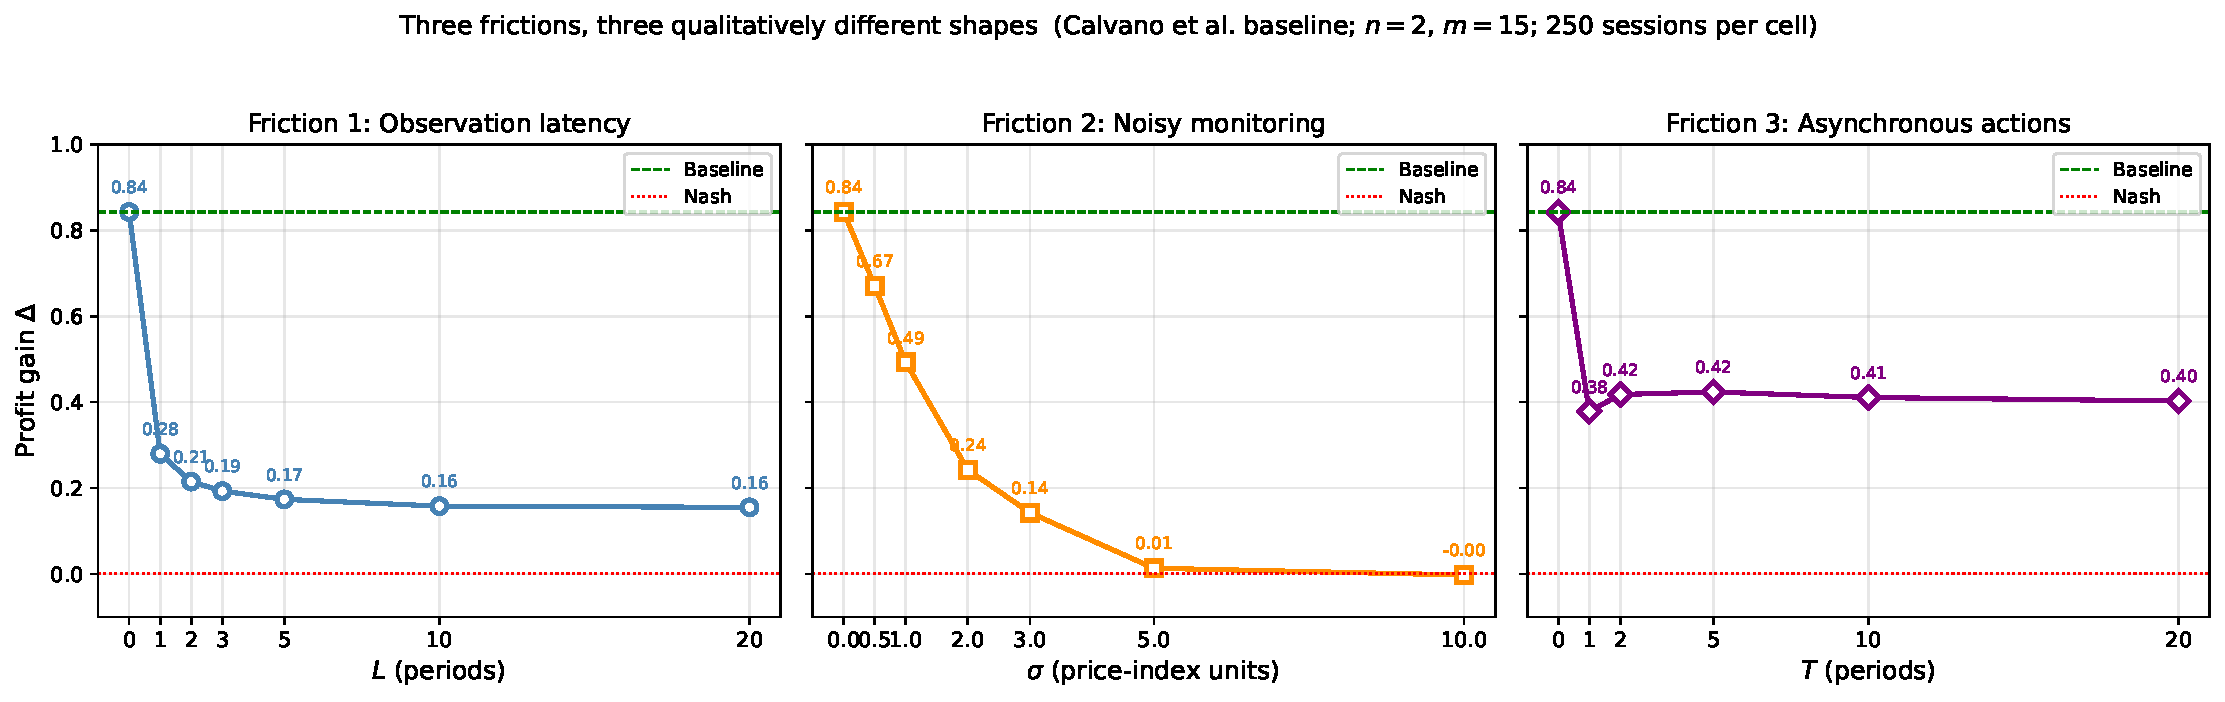
\includegraphics[width=0.99\linewidth]{figures/fig_three_friction_comparison.pdf}
\caption{Three frictions, three qualitatively different shapes. Latency: cliff at $L=1$ then floor at $\Delta\approx 0.16$. Noise: smooth monotone decline to Nash. Asynchrony: step from baseline at $T=0$ to plateau at $\Delta\approx 0.41$.}
\label{fig:three-friction}
\end{figure}

The three shapes correspond to three distinct mechanisms by which information or timing structure can interfere with learned collusion. \emph{Latency} delays signals; \emph{noise} corrupts them; \emph{asynchrony} restructures the game. Each leaves the others intact, which makes them natural candidates for a factorial test.

\section{Results: combined frictions}
\label{sec:results-factorial}

\subsection{Design recap and benchmark predictions}
\label{sec:factorial-design-recap}

The factorial described in Section~\ref{sec:methodology-combined} crosses all three frictions at two levels each:
\begin{align*}
    L \in \{0,\, 2\}, \qquad
    \sigma \in \{0,\, 1\}, \qquad
    T \in \{0,\, 1\}.
\end{align*}
The eight cells $\texttt{F}abc$ ($a,b,c \in \{0,1\}$) span every combination. Each cell was run at three replication sizes ($N\in\{250,500,1000\}$ sessions) to confirm that the interaction pattern is stable to sampling noise.

For each multi-friction cell we compare the observed $\Delta$ against three benchmark predictions:
\begin{description}[leftmargin=2.4em, style=nextline]
    \item[Additive] $\widehat{\Delta}_{\mathrm{add}} \;=\; \max\!\bigl\{0,\; \Delta_{0} - \sum_{i\in\mathcal{F}} \bigl(\Delta_{0} - \Delta_{i}\bigr)\bigr\}$, where $\mathcal{F}$ is the set of frictions ``on'' in the cell, $\Delta_0$ the baseline, and $\Delta_i$ the corresponding single-friction value.
    \item[Multiplicative] $\widehat{\Delta}_{\mathrm{mult}} \;=\; \Delta_{0} \cdot \prod_{i\in\mathcal{F}} \Delta_{i}/\Delta_{0}$.
    \item[Minimum] $\widehat{\Delta}_{\mathrm{min}} \;=\; \min_{i\in\mathcal{F}} \Delta_{i}$ --- the most-destructive single friction wins.
\end{description}
The additive prediction is the naive ``effects add'' benchmark and is clearly wrong at the extremes (sums of $>100\%$ reductions are nonsense), but it is reported for completeness because it is the prediction one would write down without thinking carefully. The multiplicative prediction treats each friction's relative damage to $\Delta$ as an independent dampening factor. The minimum prediction is the prediction one would make if frictions did not interact at all and the strongest one entirely determined the outcome.\todo{Consider also reporting a ``maximum'' prediction (collusion is preserved up to the level of the weakest friction). Symmetric to ``minimum'' in spirit; could be a complementary comparison point.}

\subsection{Cross-validation of the unified implementation}
\label{sec:factorial-crosscheck}

Four cells of the factorial constitute internal cross-validation against the single-friction implementations of Section~\ref{sec:results-singles}, since they correspond to inputs at which the unified learner should reproduce the corresponding single-friction learner exactly:
\begin{itemize}[topsep=0pt, itemsep=2pt]
    \item \texttt{F000} $(0,0,0)$: should reproduce the baseline.
    \item \texttt{F100} $(2,0,0)$: should reproduce the latency-only cell at $L=2$.
    \item \texttt{F010} $(0,1,0)$: should reproduce the noise-only cell at $\sigma=1$.
    \item \texttt{F001} $(0,0,1)$: should reproduce the async-only cell at $T=1$.
\end{itemize}

Table~\ref{tab:factorial-crosscheck} compares the four cells of the unified factorial against the corresponding single-friction runs. The factorial cells reproduce the single-friction values to five decimal places, providing strong evidence that the unified learner correctly composes the three frictions.

\begin{table}[H]
\centering
\caption{Cross-validation: unified factorial cells reproduce single-friction results.}
\label{tab:factorial-crosscheck}
\begin{tabular}{lcc}
\toprule
Cell                       & Single-friction $\Delta$ & Factorial $\Delta$ \\
\midrule
\texttt{F000} (baseline)   & $0.84280$ & $0.84280$ \\
\texttt{F100} ($L=2$)      & $0.21490$ & $0.21490$ \\
\texttt{F010} ($\sigma=1$) & $0.49269$ & $0.49269$ \\
\texttt{F001} ($T=1$)      & $0.37833$ & $0.37833$ \\
\bottomrule
\end{tabular}
\end{table}

\subsection{Headline results at \texorpdfstring{$N=1000$}{N=1000}}
\label{sec:factorial-headline}

Table~\ref{tab:factorial-1000} reports all eight cells at the highest replication size ($N=1000$ sessions per cell). Figure~\ref{fig:factorial-forest} renders the same data as a forest plot against the three benchmark predictions. The $N=250$ and $N=500$ replications appear in Section~\ref{sec:factorial-stability}.

\begin{table}[H]
\centering
\caption{$2\times 2\times 2$ factorial at $N=1000$ sessions per cell. SD is the cross-session standard deviation of $\Delta$. $\widehat{\Delta}_{\mathrm{add}}$, $\widehat{\Delta}_{\mathrm{mult}}$ and $\widehat{\Delta}_{\mathrm{min}}$ are the additive, multiplicative and minimum benchmark predictions of Section~\ref{sec:factorial-design-recap}.}
\label{tab:factorial-1000}
\renewcommand{\arraystretch}{1.05}
\begin{tabular}{lcccccc}
\toprule
Cell & $(L,\sigma,T)$ & $\Delta$ (obs.) & SD & $\widehat{\Delta}_{\mathrm{add}}$ & $\widehat{\Delta}_{\mathrm{mult}}$ & $\widehat{\Delta}_{\mathrm{min}}$ \\
\midrule
\texttt{F000} & $(0,0,0)$ & $0.848$ & $0.109$ & ---     & ---     & ---     \\
\texttt{F100} & $(2,0,0)$ & $0.210$ & $0.122$ & ---     & ---     & ---     \\
\texttt{F010} & $(0,1,0)$ & $0.500$ & $0.298$ & ---     & ---     & ---     \\
\texttt{F001} & $(0,0,1)$ & $0.383$ & $0.111$ & ---     & ---     & ---     \\
\midrule
\texttt{F110} & $(2,1,0)$ & $0.059$ & $0.080$ & $0.000$ & $0.124$ & $0.210$ \\
\texttt{F101} & $(2,0,1)$ & $0.346$ & $0.174$ & $0.000$ & $0.094$ & $0.210$ \\
\texttt{F011} & $(0,1,1)$ & $0.280$ & $0.103$ & $0.034$ & $0.226$ & $0.383$ \\
\texttt{F111} & $(2,1,1)$ & $0.537$ & $0.135$ & $0.000$ & $0.056$ & $0.210$ \\
\bottomrule
\end{tabular}
\end{table}

\begin{figure}[H]
\centering
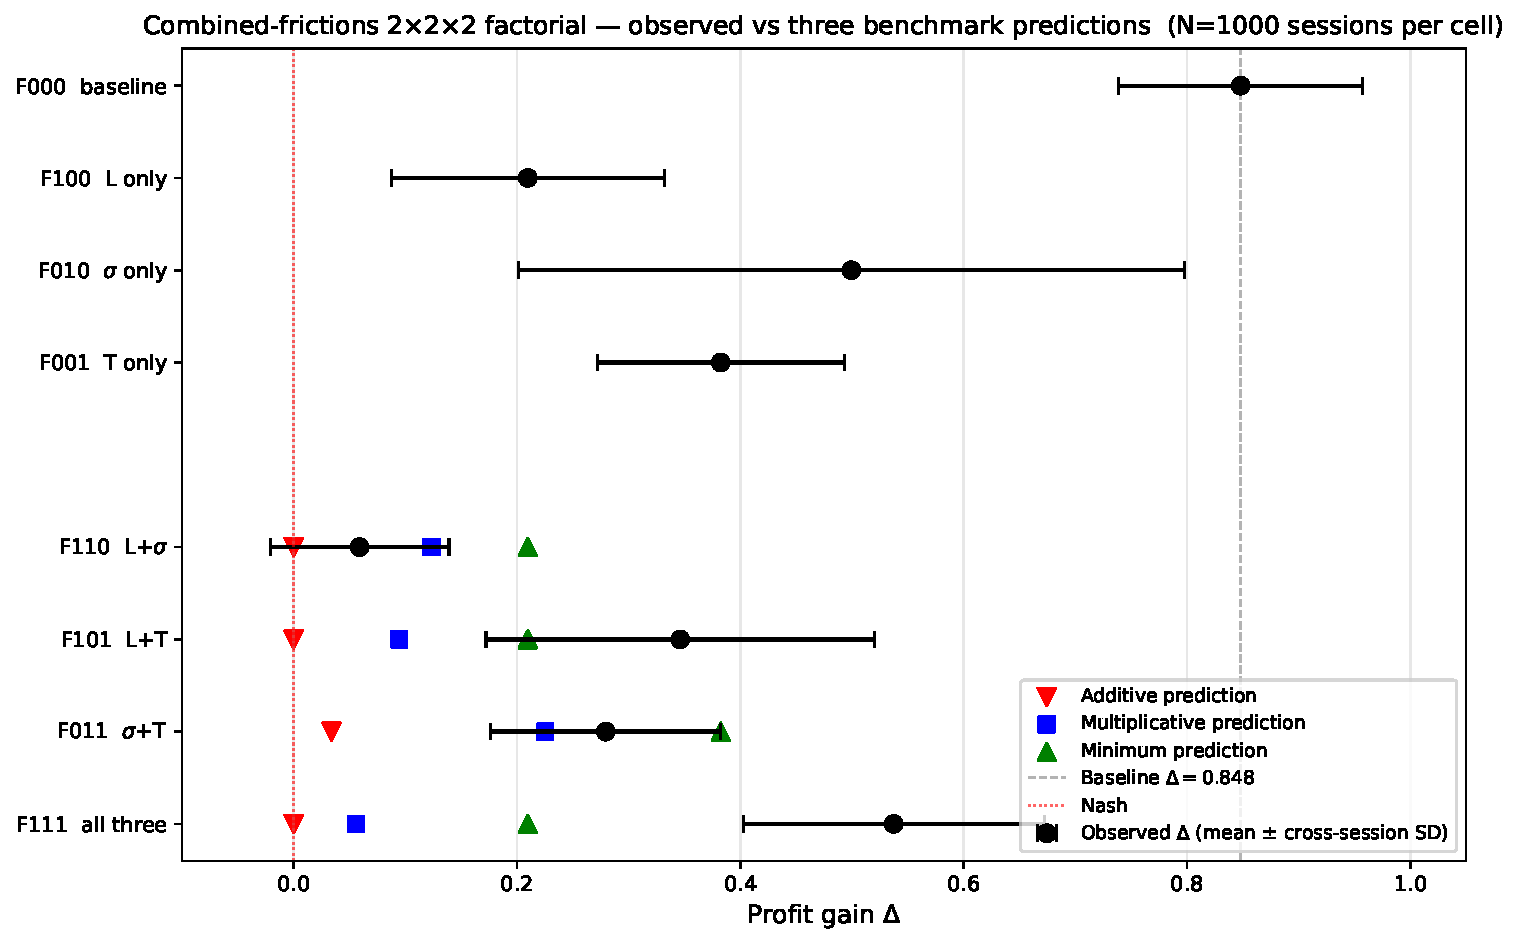
\includegraphics[width=0.95\linewidth]{figures/fig_factorial_forest.pdf}
\caption{Combined-frictions $2\times 2\times 2$ factorial at $N=1000$. Black points: observed $\Delta$; horizontal bars: cross-session SD. Coloured markers: additive (red), multiplicative (blue) and minimum (green) benchmark predictions for each multi-friction cell.}
\label{fig:factorial-forest}
\end{figure}

The four interesting cells are the four below the rule in Table~\ref{tab:factorial-1000}. Each tells a different story.

\subsubsection*{F110 (latency $+$ noise) --- super-multiplicative compounding}
The observed $\Delta = 0.059$ is below the multiplicative prediction of $0.124$ and well below the minimum prediction of $0.210$. Combining moderate latency with moderate noise destroys more of the collusion than either friction's relative effect would suggest if their dampenings were independent. The two frictions act on different dimensions of the rival-side observation --- latency on its time of arrival, noise on its value --- and stacking them produces a signal that is both stale and wrong, which is more disruptive to learning than either error alone.

\subsubsection*{F011 (noise $+$ async) --- approximately multiplicative}
The observed $\Delta = 0.280$ is reasonably close to the multiplicative prediction of $0.226$, though somewhat above it. The closeness is interesting: this is the only multi-friction cell where the multiplicative model is approximately correct.

\subsubsection*{F101 and F111 --- async ``rescues'' collusion}
The two cells with $T=1$ on top of latency (\texttt{F101}, \texttt{F111}) tell the most surprising story. \texttt{F101} ($L=2$, $T=1$) yields $\Delta = 0.346$, \emph{higher} than the latency-only cell \texttt{F100} ($\Delta = 0.210$). Adding asynchrony on top of latency \emph{increases} collusion. The same pattern is even more pronounced in the all-frictions cell \texttt{F111}: $\Delta = 0.537$ is higher than \texttt{F110} ($\Delta = 0.059$, latency $+$ noise alone), and indeed higher than every multi-friction cell that lacks asynchrony.

This is an opposite-sign interaction: asynchrony alone reduces $\Delta$ from $0.848$ to $0.383$, but adding asynchrony on top of latency (or latency-and-noise) increases $\Delta$ relative to those baselines. The mechanism story we tentatively offer is that strict alternation imposes a one-period structural commitment on the moving agent's rival, providing the moving agent with a stable target against which to optimise. When the rival's signal is itself corrupted (by noise) or stale (by latency), this structural commitment partially substitutes for the missing information. The agents can coordinate on the commitment schedule itself rather than on the agent's strategy, which is unobservable through the corrupted signal.\todo{This mechanism story is plausible but speculative. Off-path deviation analysis (sensu \citealp{calvano2023}) would help adjudicate: do the F101 and F111 strategies support genuine punishment, or are they spurious focal-point equilibria? Add this to limitations / future work.}

\subsection{Stability across replication sizes}
\label{sec:factorial-stability}

A natural concern is that the headline pattern --- particularly $\Delta_{\texttt{F111}} > \Delta_{\texttt{F110}}$ and $\Delta_{\texttt{F101}} > \Delta_{\texttt{F100}}$ --- could be sampling noise. Table~\ref{tab:factorial-acrossN} reports all eight cells at $N\in\{250,500,1000\}$.

\begin{table}[H]
\centering
\caption{Factorial $\Delta$ across replication sizes. Movements between columns are within sampling noise; the qualitative pattern is identical at all three $N$.}
\label{tab:factorial-acrossN}
\renewcommand{\arraystretch}{1.05}
\begin{tabular}{lccc}
\toprule
Cell & $\Delta\;(N{=}250)$ & $\Delta\;(N{=}500)$ & $\Delta\;(N{=}1000)$ \\
\midrule
\texttt{F000} & $0.843$ & $0.842$ & $0.848$ \\
\texttt{F100} & $0.215$ & $0.212$ & $0.210$ \\
\texttt{F010} & $0.493$ & $0.496$ & $0.500$ \\
\texttt{F001} & $0.378$ & $0.385$ & $0.383$ \\
\texttt{F110} & $0.063$ & $0.062$ & $0.059$ \\
\texttt{F101} & $0.323$ & $0.343$ & $0.346$ \\
\texttt{F011} & $0.264$ & $0.277$ & $0.280$ \\
\texttt{F111} & $0.551$ & $0.539$ & $0.537$ \\
\bottomrule
\end{tabular}
\end{table}

\begin{figure}[H]
\centering
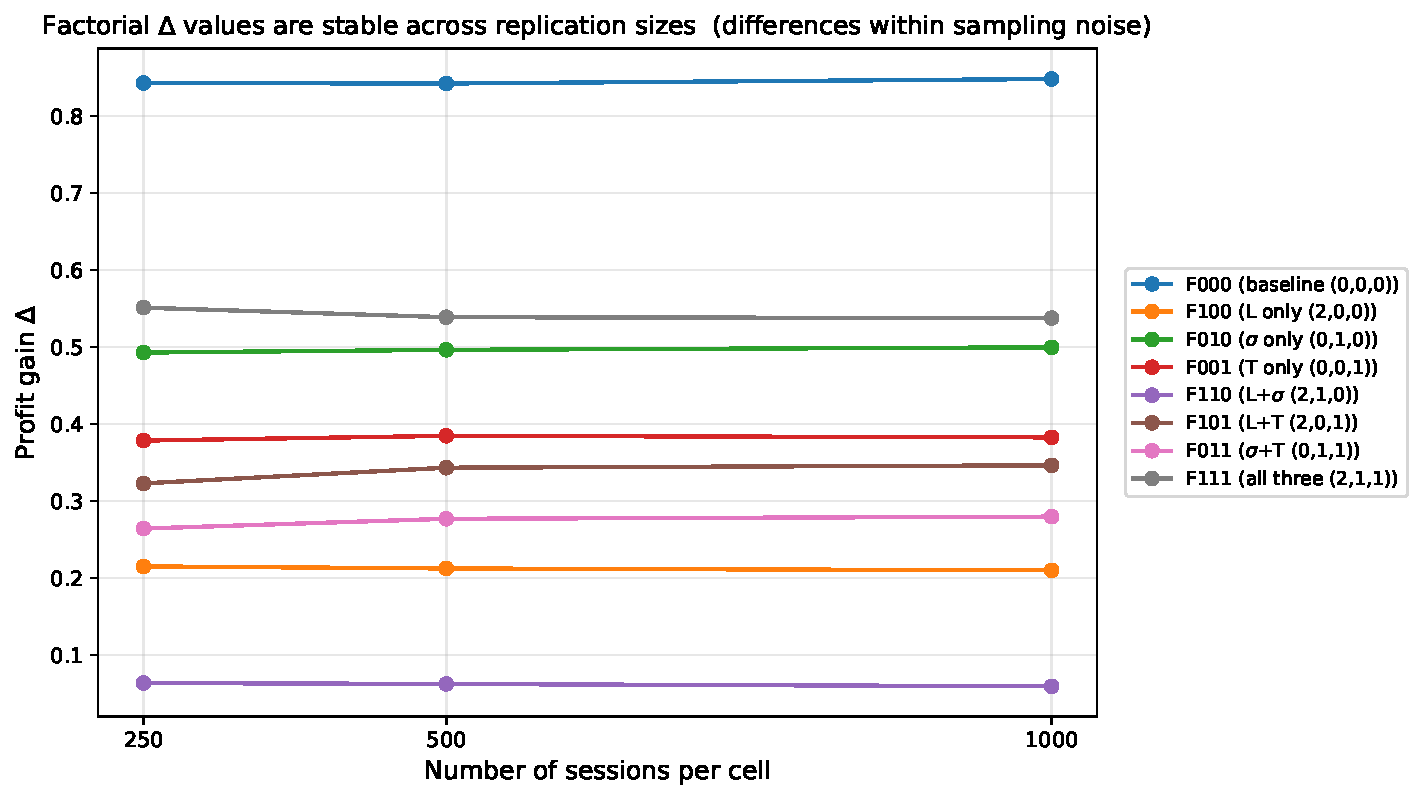
\includegraphics[width=0.95\linewidth]{figures/fig_factorial_acrossN.pdf}
\caption{Factorial $\Delta$ values at $N\in\{250,500,1000\}$ for all eight cells. The observed pattern is qualitatively identical across replication sizes, with cell-level movements between $N$'s typically below $0.02$.}
\label{fig:factorial-acrossN}
\end{figure}

The cell-level $\Delta$ values move by less than $0.025$ between $N=250$ and $N=1000$. The headline interaction patterns --- super-multiplicative compounding of $L$ and $\sigma$, async rescuing collusion in \texttt{F101} and \texttt{F111} --- are visually identical at all three replication sizes. The standard error of the mean across sessions, $\mathrm{SD}/\sqrt{N}$, is approximately $0.004$ at $N=1000$ on the headline cells, well below any of the inter-cell differences that drive the interpretation. We therefore consider the interaction pattern robust to sampling noise.

\subsection{Summary of factorial findings}
\label{sec:factorial-summary}

Three findings emerge that survive replication and that we carry into the discussion:
\begin{enumerate}[topsep=2pt, itemsep=2pt]
    \item Latency and noise compound \emph{super-multiplicatively}.
    \item Asynchrony, in combination with either latency or noise (or both), \emph{partially restores} collusion that the other frictions would otherwise destroy --- an opposite-sign interaction with respect to the main effect of asynchrony.
    \item No single benchmark prediction (additive, multiplicative, or minimum) describes all four multi-friction cells. The factorial therefore rejects the simplest models of how frictions ought to combine.
\end{enumerate}

\section{Discussion}
\label{sec:discussion}

\subsection{Synthesising the three single-friction shapes}
\label{sec:discussion-shapes}

The single-friction sweeps in Section~\ref{sec:results-singles} produced three qualitatively different $\Delta(\cdot)$ curves. The shapes are not arbitrary; each maps to a distinct mechanism by which information or timing structure interferes with what the Q-learners are learning.

\paragraph{Latency: a cliff plus a floor.} Observation latency causes the largest disruption at $L=1$ (a sixty-seven-percent drop) and very little additional disruption thereafter. The cliff is consistent with the architecture of the Calvano agents: their state is the rival's last-period price, and their learnt strategies condition on that state. Severing the link between the period the rival actually played a price and the period in which the agent learns about that price destroys conditioning, reward, and punishment all at once. The size of the cliff is therefore not surprising. The residual at $\Delta\approx 0.16$ for $L\geq 5$ is. It implies that some component of learned collusion does not require timely monitoring at all --- the agents converge on a focal mutual-high-price that is sustained without enforcement. We return to this when interpreting the factorial: the residual $0.16$ floor disappears when noise is added, suggesting noise destroys precisely this focal-point mechanism.

\paragraph{Noise: smooth decline, no floor.} The noise curve is smooth and monotone: $\Delta$ falls continuously from $0.84$ at $\sigma=0$ to indistinguishable-from-Nash by $\sigma=5$. There is no residual floor. The mechanism story differs from latency. With noise, the rival's signal arrives on time but is wrong; at high $\sigma$, the perceived rival-side state is near-independent of the rival's actual price, and any policy that conditions on that perceived state encodes no rival-relevant information. Both reactive collusion (latency-style punishment) and focal-point collusion (the residual under heavy latency) require that the perceived state contain rival-side information; noise destroys both, hence no floor.

\paragraph{Asynchrony: step then plateau.} Strict alternation cuts $\Delta$ in half from $T=0$ to $T=1$ and produces no further movement for $T\geq 2$. The drop is structural --- it depends on \emph{whether} prices are simultaneous or staggered, not much on \emph{how} staggered they are. Two explanations are consistent with the data. First, half-rate state-visitation: with strict alternation, each agent observes only half as many state-action transitions per unit of calendar time, so its learning is correspondingly less coverage-rich. Second, a strategic explanation along Maskin--Tirole lines: the equilibrium set of the alternating-move game differs from that of the simultaneous game, and the equilibrium that Q-learners select in the alternating-move game happens to be lower. The two explanations make different predictions: the first predicts that doubling the iteration budget (doubling effective coverage) would close the gap, while the second does not. Distinguishing them is left to future work.

\subsection{Why latency and noise compound super-multiplicatively}
\label{sec:discussion-LxNoise}

The factorial result $\Delta_{\texttt{F110}} = 0.059$, below both the multiplicative prediction ($0.124$) and the minimum prediction ($0.210$), is the strongest evidence in this paper for non-trivial interaction. The mechanism story we offer is that latency and noise act on different dimensions of the rival-side observation: latency on its time-of-arrival, noise on its value. Either dimension alone leaves some learning signal intact: under pure latency, the value is correct (just stale, useful for focal-point coordination); under pure noise, the timing is correct (so an agent can in principle de-noise across many observations, though the Q-learner does not actually do this). Combined, neither the time-of-arrival nor the value is reliable. The signal is both stale and wrong, and the residual focal-point coordination that survives in the latency-only case is destroyed by the noise component. The two single-friction effects are not independent dampenings but jointly compound, eliminating different parts of the learning machinery.

This is consistent with the observation in Section~\ref{sec:discussion-shapes} that the latency-only $\Delta\approx 0.16$ floor presumably reflects focal-point coordination that does not require timely monitoring. Adding noise destroys precisely that focal-point mechanism, which is why the joint cell falls to near-Nash even though latency alone left some collusion.

\subsection{Why asynchrony rescues collusion in combination}
\label{sec:discussion-async-rescue}

The most surprising finding is that asynchrony, despite reducing $\Delta$ in isolation, partially \emph{restores} $\Delta$ when imposed jointly with latency or noise. This is an opposite-sign interaction --- the same intervention has different signs as a stand-alone modification versus as an addition to an already-frictional environment.

The mechanism we tentatively propose is that strict alternation imposes a one-period structural commitment on whichever agent moved last. The agent currently moving therefore faces a known, locked-in rival price. When the rival-side signal is otherwise corrupted (by noise) or stale (by latency), this structural commitment partially substitutes for what the moving agent would otherwise have to infer from a low-quality signal. Coordination shifts from being about ``what is the rival's strategy, given a noisy/lagged read on what they did?'' to being about ``the rival is locked in for one more period, what is my best response?''. The latter problem is much easier because the rival's price is given by the institutional schedule, not by the algorithm's strategy.

If this story is right, the rescue is not unbounded: once the structural commitment becomes too long to be useful for short-horizon coordination ($T \gg 1$), or once the underlying frictions become too severe even for an agent that observes the rival's commitment to overcome, the rescue should weaken or vanish. Our factorial holds $T$ at one and varies only the others. A natural follow-up would scan $T$ at the joint $(L,\sigma)$ levels and see how the rescue scales.

A competing explanation, less attractive, is that the rescue is a learning-stability artefact rather than a strategic effect: the alternation schedule reduces the joint action space the algorithm has to explore at each step, so under high $L+\sigma$ noise the alternation makes the underlying learning problem more tractable. Off-path deviation tests would help adjudicate, and we list them as priority future work in Section~\ref{sec:limitations}.

\subsection{Implications for policy}
\label{sec:discussion-policy}

\citet{zhang2025} argues that injecting noise into the rival-price signal could be a regulatory tool against algorithmic collusion. The single-friction result of Section~\ref{sec:results-noise} is broadly consistent with this view: noise alone does drive $\Delta$ to Nash, given a sufficiently large $\sigma$. The factorial qualifies the conclusion in two ways.

First, noise injection is more effective when latency is also present: $\Delta_{\texttt{F110}} = 0.059$ versus $\Delta_{\texttt{F010}} = 0.500$. A regulator who can mandate a small observation delay alongside a noise-injection rule will achieve more decisive collusion-disruption than either rule alone, and more than the additive or multiplicative naive predictions would imply. The two information frictions are policy \emph{complements}.

Second, structural-timing interventions (mandated staggered pricing windows) appear to be policy \emph{substitutes} for information-degradation interventions in the sense that the structural-timing rule \emph{undoes} part of the information-degradation rule's effect on collusion. A regulator who imposes alternating-price-window rules \emph{and} noise-injection rules at the same time gets less collusion-disruption from the noise rule than they would have gotten without the alternation rule. This is the opposite of the additive-effects intuition that one might bring to combinatorial regulatory design.

The bottom line is that the policy-relevant outcome is not the sum or product of single-friction analyses. Combinations of information and timing rules need to be evaluated jointly, ideally on the same Q-learning environment that motivates the policy concern.\todo{The policy paragraphs above lean on a single $(L,\sigma,T)$ point in the factorial. Before relying on them in the final draft, ideally re-do the experiment at one or two more $(L,\sigma)$ levels; the heatmaps suggested in future work would do this directly.}

\subsection{Relation to the prior literature}
\label{sec:discussion-relation-to-lit}

The single-friction results both confirm and refine the prior literature.

\citet{calvano2021} find that imperfect monitoring (in their Cournot setting, via stochastic demand) reduces but does not eliminate algorithmic collusion at moderate noise levels. Our noise sweep is qualitatively consistent: at $\sigma=0.5$ and $\sigma=1$, $\Delta$ remains substantially above Nash; only at $\sigma\geq 5$ does it fall to indistinguishable-from-Nash. That said, a quantitative comparison is not appropriate: the demand structures and noise specifications differ.

\citet{klein2021} finds that Q-learners in alternating-move pricing converge on supracompetitive prices, sometimes via Edgeworth-cycle dynamics. Our async result is in a different sign than naive reading of Klein would suggest --- alternation in our setting reduces $\Delta$ rather than preserves it. The two results are not directly contradictory: Klein uses sequential pricing as the base game, with the algorithm trained from random initial Q on that game, whereas we impose alternation as a friction on top of the simultaneous baseline. The two questions are different (``what does the algorithm converge to in the alternating-move game?'' vs ``what happens if we suddenly impose alternation on agents that would otherwise play a simultaneous game?''). Our result is the second.

\citet{calvano2023} ask whether high prices are genuine (sustained by learnt punishment) or spurious (artefacts of action selection). Our paper does not run their off-path tests, so we cannot say which of our high-$\Delta$ cells are genuine in their sense. The async-rescue cells (\texttt{F101}, \texttt{F111}) are particularly interesting candidates for this test, because the mechanism story we offer (structural commitment substituting for signal quality) would predict the rescue to survive deviations more reliably than reactive punishment would. We list this as a priority extension.

\citet{zhang2025}'s noise-injection policy proposal is consistent with our single-friction results but, as noted in Section~\ref{sec:discussion-policy}, the factorial qualifies the case for the policy: in the presence of latency, noise injection is more effective than Zhang predicts; in the presence of asynchrony, less.

\section{Limitations and next steps}
\label{sec:limitations}

The design of this thesis is deliberately controlled: it keeps the Calvano pricing environment fixed and varies only the information and timing frictions. That is the source of the main contribution, because it makes the interaction effects interpretable. It also sets the boundary of what the results can claim. The thesis identifies mechanisms inside a stylised Q-learning environment; it does not provide a market-by-market quantitative forecast.

\begin{itemize}[topsep=2pt, itemsep=4pt]
    \item \textbf{Asymmetric and heterogeneous frictions.} All three frictions are imposed symmetrically on the two agents. Real markets often feature asymmetric frictions, for example one firm with a faster price-update cadence, cleaner data feed, or stronger scraping infrastructure than the other. \citet{brown2023}'s empirical findings on asymmetric update frequencies make this the most natural next extension.
    \item \textbf{A homogeneous two-firm product environment.} The model keeps the two firms symmetric in appeal and cost, with differentiation entering through the logit demand system. This is useful for isolating the learning mechanism, but it leaves out richer market structure: more firms, asymmetric costs, product-level heterogeneity, capacity constraints, and consumer search frictions.
    \item \textbf{Bounded memory and richer algorithms.} Appendix~\ref{app:bounded-memory} explains why extending tabular Q-learning from one-period memory to two-period memory is computationally demanding in this state space. A meaningful extension would require either substantially larger compute, for example a high-performance-computing allocation, or a methodological switch to function-approximated $Q$. That step would also allow comparison with more modern pricing algorithms, but at the cost of giving up the transparent tabular mechanism used here.
\end{itemize}

These limitations do not undermine the main result. They point to where the mechanism should be stress-tested next: asymmetric firms, richer product environments, and learning rules with more memory. The central finding remains that information and timing frictions cannot be evaluated one at a time, because their combination can qualitatively change the degree of learned collusion.


\bibliographystyle{abbrvnat}
\bibliography{references}

\appendix
\section{Implementation details}
\label{app:implementation}

\subsection{Code structure}

The C++ simulator lives in \texttt{Code/ogcode/cpp\,conversion/} and is structured around four executables, each sharing a common library of routines:
\begin{itemize}[itemsep=2pt, topsep=2pt]
    \item \texttt{ogcode\_cpp.exe} --- baseline learner (no frictions).
    \item \texttt{ogcode\_latency.exe} --- latency-only learner; reads \texttt{A\_Latency.txt}.
    \item \texttt{ogcode\_noise.exe} --- noise-only learner; reads \texttt{A\_NoiseStd.txt}.
    \item \texttt{ogcode\_async.exe} --- asynchronous-actions learner; reads \texttt{A\_LockIn.txt}.
    \item \texttt{ogcode\_combined.exe} --- unified learner accepting all three friction parameters.
\end{itemize}
The single-friction binaries exist primarily for cross-validation against the unified one. Each defaults its non-applicable friction parameters to zero, so at all-zero inputs every binary reproduces the baseline bit-for-bit. This is the principal correctness check.

The unified \texttt{LearningSimulationCombined.cpp} is the implementation actually used for the factorial. The order of operations within an iteration mirrors the description in Section~\ref{sec:methodology-combined}: (1) compute per-agent perceived state with fresh Gaussian noise on the latency-lagged opponent observation, (2) determine the moving agent under $T$-period lock-in, (3) action selection on the perceived state for the moving agent (non-mover repeats their previous price), (4) compute the true joint reward, (5) Q-update each agent on its own perceived state, (6) advance buffers.

\subsection{Random number generation and reproducibility}

The Calvano reference code uses a Numerical-Recipes \texttt{Ran2}-style generator for exploration draws and Q-initialisation tie-breaking. Our translation preserves that generator and its seeding convention so that at zero-friction inputs the unified learner reproduces the baseline exactly. Gaussian noise (Friction~2) uses an independent \texttt{std::mt19937\_64} stream seeded deterministically from the session index. At $\sigma=0$ the noise stream is short-circuited and never advanced, which guarantees that the baseline is reproduced bit-for-bit when noise is off, regardless of how the noise stream is configured.

\section{Design choices not specified in the proposal}
\label{app:design-choices}

This appendix collects every implementation-level decision that the proposal underspecified or where the implementation deliberately departs from the proposal's wording. Each is justified briefly.

\paragraph{Friction~2 noise distribution.}
The proposal specified a discrete-flip noise model: with probability $q$, the rival's observed price index is perturbed to a neighbouring grid point. The implemented version is a Gaussian-on-index model (Equation~\ref{eq:noise}). The Gaussian model is a one-parameter generalisation: at $\sigma=0$ it is the no-noise baseline, at small $\sigma$ it produces small deviations to nearby indices (so it locally agrees with the discrete-flip intuition), and at large $\sigma$ it converges on near-uniform random observation. The discrete-flip variant remains a future-work item.

\paragraph{Friction~3 alternation schedule.}
The proposal specified ``alternating or random selection'' for which agent moves each period; the implemented version uses strict deterministic alternation with a tunable lock-in length $T$ (Section~\ref{sec:methodology-async}). Strict alternation matches the canonical Maskin--Tirole specification and is invariant to RNG state, simplifying cross-validation. Random alternation remains a future-work item.

\paragraph{Off-path deviation tests.}
The proposal specified off-path deviation tests for the asynchronous case as a way to distinguish genuine collusion from timing artefacts. The implemented version does not include them. They are listed as priority extensions in Section~\ref{sec:lim-method}.

\paragraph{Noise on price index, not on price value.}
Equation~\ref{eq:noise} adds noise to the price index $k_j\in\{1,\dots,m\}$ rather than to the price value $p_j$ in money units. The two differ by a multiplicative factor (the spacing of the grid). The index-space convention has the advantage that $\sigma$ has a transparent ``noise in number of grid steps'' interpretation, and the friction parameter is independent of the choice of price grid. In the price-value convention $\sigma$ would have to be re-scaled when the grid changes.

\paragraph{Per-agent noise draws.}
Each agent draws its own independent Gaussian noise each period. Correlated noise across agents (a common shock to monitoring) is a different story (it overlaps with the literature on common observation errors); we do not pursue it here.

\paragraph{Both agents update Q under asynchrony.}
Under strict alternation only the moving agent revises its action. The implementation has both agents Q-update each period regardless of who moved (Section~\ref{sec:methodology-async}). The non-mover's ``action'' is its previous-period price, which is a valid element of its action set, and the non-mover observes the actual joint reward. Discarding the non-mover's update would discard a legitimate learning signal.

\paragraph{Initial-period buffer initialisation.}
The latency buffer of length $L+1$ per agent is filled at session start by repeating the agent's randomly drawn initial price across all slots, rather than by drawing $L+1$ independent initial prices. Repetition is chosen for simplicity; during the first $L$ iterations of every session the exploration probability $\varepsilon\approx 1$, so the buffer contents are essentially overwritten by random exploration before they affect any learnt policy.

\section{Numerical results in full}
\label{app:numerics}

\subsection{Single-friction sweeps}

Tables~\ref{tab:latency-results}, \ref{tab:noise-results} and \ref{tab:async-results} in Section~\ref{sec:results-singles} are the canonical numerical results for the three single-friction sweeps. All values are means of converged session-level $\Delta$, with cross-session standard deviation reported alongside.

\subsection{Grid-robustness check}

Table~\ref{tab:grid-robustness} reports $\Delta$ at four grid sizes $m\in\{15,25,50,100\}$ on the otherwise-identical Calvano baseline (no frictions). The $m=15$ and $m=25$ runs use $1{,}000$ sessions; $m=50$ and $m=100$ use $250$ sessions to keep runtime feasible on a local workstation. The $m=100$ runs additionally use a 5{,}000-episode convergence cap rather than $1{,}000$, since the larger state space takes longer to converge.

\begin{table}[H]
\centering
\caption{Grid-robustness check. $\Delta$ falls modestly with finer price grid but plateaus by $m=50$ and is essentially unchanged from $m=50$ to $m=100$. All runs use Calvano's original fixed-$\beta$ protocol.}
\label{tab:grid-robustness}
\begin{tabular}{rcccc}
\toprule
$m$ & sessions & $\Delta$ & SD & avg time-to-convergence \\
\midrule
15  & 1000 & 0.848 & 0.109 & 261 episodes  \\
25  & 1000 & 0.806 & 0.076 & 364 episodes  \\
50  & 250  & 0.707 & 0.023 & 476 episodes  \\
100 & 250  & 0.706 & 0.016 & 1144 episodes \\
\bottomrule
\end{tabular}
\end{table}

The $\nu$-corrected version of this check, in which $\beta$ is scaled with $m$ to hold expected per-cell visit count constant per Equation~\ref{eq:nu-visit-count}, is left for future work. Without that correction it is conceivable that some of the $\Delta$ decline from $m=15$ to $m=100$ reflects worse exploration per cell rather than a genuine effect of the finer grid; with the correction the comparison would be cleaner.\todo{Run the $\nu$-corrected version on the cluster as part of the same job set as the pairwise heatmaps. Calvano (2020, Section 6.7) discuss this confound.}


\end{document}
